\documentclass[journal,12pt,twocolumn]{IEEEtran}
\usepackage{graphicx}
\graphicspath{{./figs/}}{}
\usepackage{amsmath,amssymb,amsfonts,amsthm}
\newcommand{\myvec}[1]{\ensuremath{\begin{pmatrix}#1\end{pmatrix}}}

\let\vec\mathbf

\title{
Matrix-Lines
}
\author{Kukunuri Sampath Govardhan}
\begin{document}
\maketitle
\tableofcontents
\bigskip
\section{Problem Statement}
Find equation of a line passing trough a point (2,2) and cutting off intercepts on the axes whose sum is 9.\\
\section{Construction}
\begin{figure}[h]
    \centering
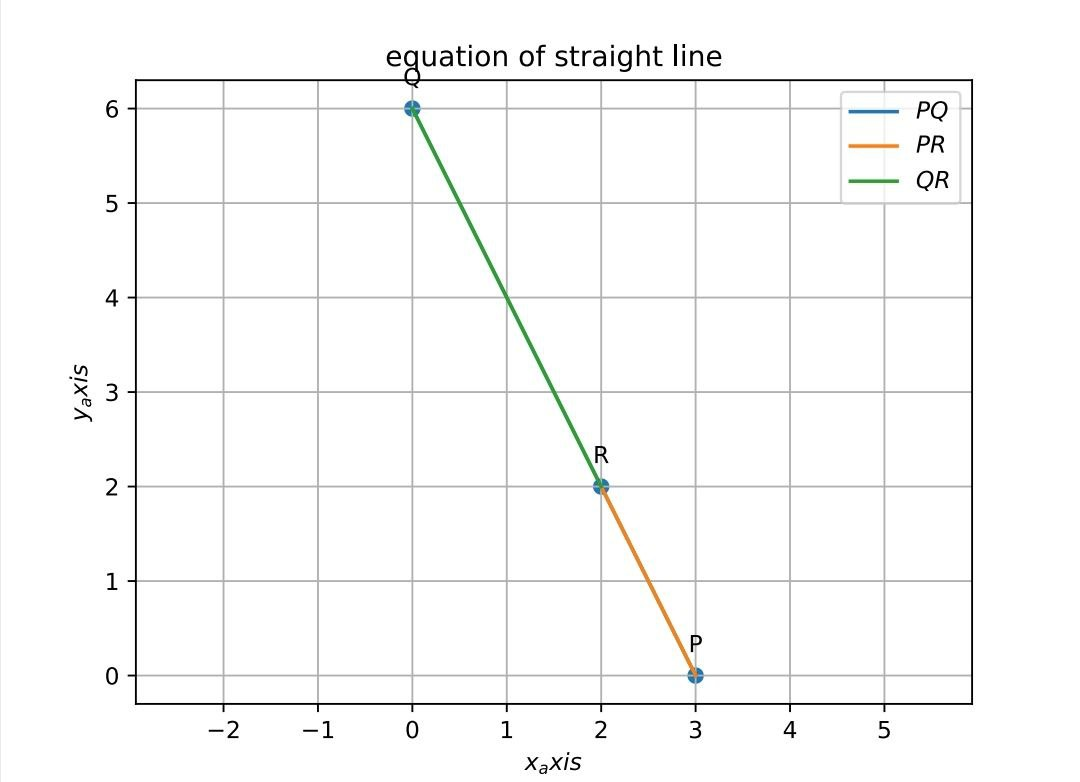
\includegraphics[width=\columnwidth]{figs/assign4.png}
    \caption{Equation of the Straight Line}
    \label{fig:my_label}
\end{figure}
\vspace{2cm}
\begin{table}[h]
    \centering
    \begin{tabular}{|c|c|c|}
       \hline
       \textbf{Symbol}&\textbf{Value}&\textbf{Description}  \\
       \hline
	    $\vec{P}$ & $\myvec{
		    a\\
		    0}$
	    & Point on X-axis\\
        \hline
	    $\vec{Q}$ & $\myvec{0\\b}$
 & Point on Y-axis\\
        \hline
	    $\vec{R}$ & $\myvec{
  2\\
  2}$
 & Given Point \\
        \hline
        a + b & 9 & Given Condition\\
        \hline
    \end{tabular}
    \caption{Parameters}
    \label{tab:my_label}
\end{table}


\section{Solution}
Given that resultant line passes through point(2,2) and intercepts on axes whose sum is 9 (let x intercept is a and y intercept is b therefore, a + b = 9 ) \\
\\
so, b = 9 - a  \\
\\
Let ${\vec{P}}$=$\myvec{
  a\\
  0}$
 , ${\vec{Q}}$=$\myvec{
  0\\
  9-a}$
  , ${\vec{R}}$=$\myvec{
  2\\
  2}$
\\
\\
Equation of line is ${\vec{n^{\top}}\vec{X}} = c$.\\
\\
Now we have 3 points which lies on same line so,\\
 The Equation of line through ${\vec{P}}$ is\\
\begin{equation}
	\vec{n^{\top}}
	\myvec{
  a\\
  0}
  = c \label{eq-1}
\end{equation}
\\
Equation of line passing through ${\vec{Q}}$ is\\
\begin{equation}
	\vec{n^{\top}}
     \myvec{
  0\\
  9 - a
 }
  = c \label{eq-2}
\end{equation}
\\
Now eq1 + eq2,\\
\begin{equation}
	\vec{n^{\top}}
	\myvec{
  a\\
  9 - a
}
  = 2c \label{eq-3}
\end{equation}
\\
Equation of line passing through ${\vec{R}}$ is\\
\begin{equation}
	\vec{n^{\top}}
	\myvec{
  2\\
  2}
  = c \label{eq-4}
\end{equation}
 \\
 From eq3 and eq4 we can find normal vector ${\vec{n}}$,\\
 \\
 \begin{equation}
	 \vec{n^{\top}}
	 \myvec{
  a & 9-a\\
  2 & 2
 }
	 = c.\myvec{
  2\\
  1}
 \label{eq-5}
\end{equation}
 \\
 Therefore,\\
 \begin{equation}
	 \vec{n^{\top}} = 
	 \myvec{
  a & 9-a\\
  2 & 2
 }
  ^{-1}
  .
	 \myvec{
  2\\
  1}
 .c \label{eq-6}
\end{equation}
 \\
\begin{equation}
	\vec{n^{\top}} = 
	\myvec{
  3a-9\\
  -2}
  .\frac{c}{4a-18}
 \label{eq-7}
\end{equation}
 \\
 Now eq4 can be expressed as,\\
 \\
  \begin{equation}
	  \myvec{
  3a - 9\\
  -2}
 .
	  \myvec{
  2\\
  2}
  .\frac{c}{4a-18} = c
 \label{eq-8}
\end{equation}
  \\
  Thus, we get \textbf{a = 2, b = 9-a = 7}\\
  \\
  by substuting a in eq6, finally\\
  \\
   \begin{equation}
	   \vec{n^{\top}} = 
	   \myvec{
  0.3\\
  0.2}
 .c
 \end{equation}
  \\
The Resultant Equation of line is ${\vec{n^{\top}}\vec{X}} = c$ \\
\\
 \begin{equation}
	 \myvec{
  0.3\\
  0.2\\
 }
	 .\vec{X}.c = c
 \end{equation}
  \\
i.e,    \\
\begin{equation}
	\myvec{
  3\\
  2}
	.\vec{X} = 10
 \end{equation}
\\
\textbf{
Therefore equation of the line is, \\
\begin{equation}
	\myvec{
  3\\
  2}
	. \vec{X} = 10
 \end{equation}}
\begin{center}
    \textbf{3x + 2y = 10}
\end{center}
\section{Software}
Download the following code using,
\begin{table}[h]
    \centering
    \begin{tabular}{|c|}
    \hline \\
         svn co https://github.com/\\mygit-sampath-govardhan/fwc-iith-assignments/blob/\\5b65abbf8e5e3c803b1bff8cf4a95092e100de75/\\Assignment-4(Matrices-line)/codes/Assignment4.py  \\
         \\
\hline
    \end{tabular}
\end{table}
\\
and execute the code by using command
\begin{center}
\textbf{Python3  Assignment4.py}\\
\end{center}

\section{Conclusion}
We found the equation of a line passing trough a point
(2,2) and cutting off intercepts on the axes whose
sum is 9.

\end{document}
